\documentclass[12pt,a4paper]{article}
\usepackage[utf8]{inputenc}
\usepackage[T1]{fontenc}
\usepackage[spanish]{babel}
\usepackage{geometry}
\usepackage{hyperref}
\usepackage{graphicx}
\usepackage{listings}
\usepackage{xcolor}
\usepackage{booktabs}
\usepackage{tabularx}
\usepackage{caption}
\usepackage{float}
\usepackage{parskip}
\usepackage{enumitem}
\usepackage{titlesec}

\geometry{margin=2.5cm}

% Cambiar "Cuadro" (babel español) por "Tabla"
\addto\captionsspanish{\renewcommand{\tablename}{Tabla}}

% Cambiar "Listing" por "Listado"
\renewcommand{\lstlistingname}{Listado}

\hypersetup{
  colorlinks=true,
  linkcolor=blue!60!black,
  urlcolor=blue!60!black,
  citecolor=blue!60!black
}

\definecolor{codegray}{rgb}{0.95,0.95,0.95}
\definecolor{codecomment}{rgb}{0.4,0.4,0.4}
\definecolor{codekeyword}{rgb}{0.0,0.3,0.7}
\definecolor{codestring}{rgb}{0.2,0.5,0.2}
\definecolor{codeannotation}{rgb}{0.6,0.3,0.0}
\definecolor{bugbg}{rgb}{1.0,0.93,0.93}
\definecolor{fixbg}{rgb}{0.93,1.0,0.93}

\lstset{
  language=Java,
  backgroundcolor=\color{codegray},
  basicstyle=\ttfamily\small,
  keywordstyle=\color{codekeyword}\bfseries,
  commentstyle=\color{codecomment}\itshape,
  stringstyle=\color{codestring},
  numbers=left,
  numberstyle=\tiny\color{gray},
  numbersep=8pt,
  breaklines=true,
  showstringspaces=false,
  frame=single,
  framerule=0pt,
  xleftmargin=1em,
  xrightmargin=0.5em,
  captionpos=b,
  extendedchars=true,
  literate=
    {á}{{\'a}}1 {é}{{\'e}}1 {í}{{\'\i}}1 {ó}{{\'o}}1 {ú}{{\'u}}1
    {Á}{{\'A}}1 {É}{{\'E}}1 {Í}{{\'I}}1 {Ó}{{\'O}}1 {Ú}{{\'U}}1
    {ñ}{{\~n}}1 {Ñ}{{\~N}}1 {ü}{{\"u}}1 {Ü}{{\"U}}1
}

\newcommand{\code}[1]{\texttt{#1}}
\newcommand{\clase}[1]{\texttt{#1}}
\newcommand{\metodo}[1]{\texttt{#1}}

\title{Corrección de bugs en el sistema de undo/redo \\
       de \texttt{PNESupport}}
\author{OpenMarkov --- org.openmarkov.core}
\date{Abril 2026}

\begin{document}

\maketitle
\tableofcontents
\newpage

% =====================================================================
\section{Introducción}
% =====================================================================

El sistema de undo/redo de OpenMarkov permite deshacer y rehacer cualquier
modificación sobre una red probabilística (\clase{ProbNet}). Toda modificación
se encapsula en un objeto \clase{PNEdit}, y el componente central que gestiona
el historial y las notificaciones a los observadores es \clase{PNESupport}.

\medskip

Cuando el usuario ejecuta una acción compuesta en la GUI ---por ejemplo, abrir
el diálogo de propiedades de un nodo, modificar varias propiedades y pulsar
Aceptar--- la GUI agrupa los edits individuales entre llamadas a
\metodo{openNewSubEditHistory()} y
\metodo{closeSubEditHistory()}.
Al cerrar, los edits se empaquetan en un \clase{ListPNEdit}
(un tipo de \clase{CompoundPNEdit}) que se trata como una unidad atómica
de undo: un solo Ctrl+Z deshace todo el grupo.

\medskip

Este mecanismo contenía \textbf{tres bugs} que afectaban tanto a las
notificaciones que reciben los listeners como al orden de ejecución de los
sub-edits. Los bugs estaban marcados con la anotación \code{@ToCheck} en el
código fuente, y llevaban tiempo sin resolverse. Este documento describe en
detalle los tres bugs, la causa raíz común, la corrección aplicada y las
pruebas que la validan.


% =====================================================================
\section{Arquitectura del sistema de undo/redo}
% =====================================================================

Antes de describir los bugs, es necesario entender la arquitectura del sistema.
La Figura~\ref{fig:arquitectura} muestra las clases implicadas y sus relaciones.

\begin{figure}[H]
  \centering
  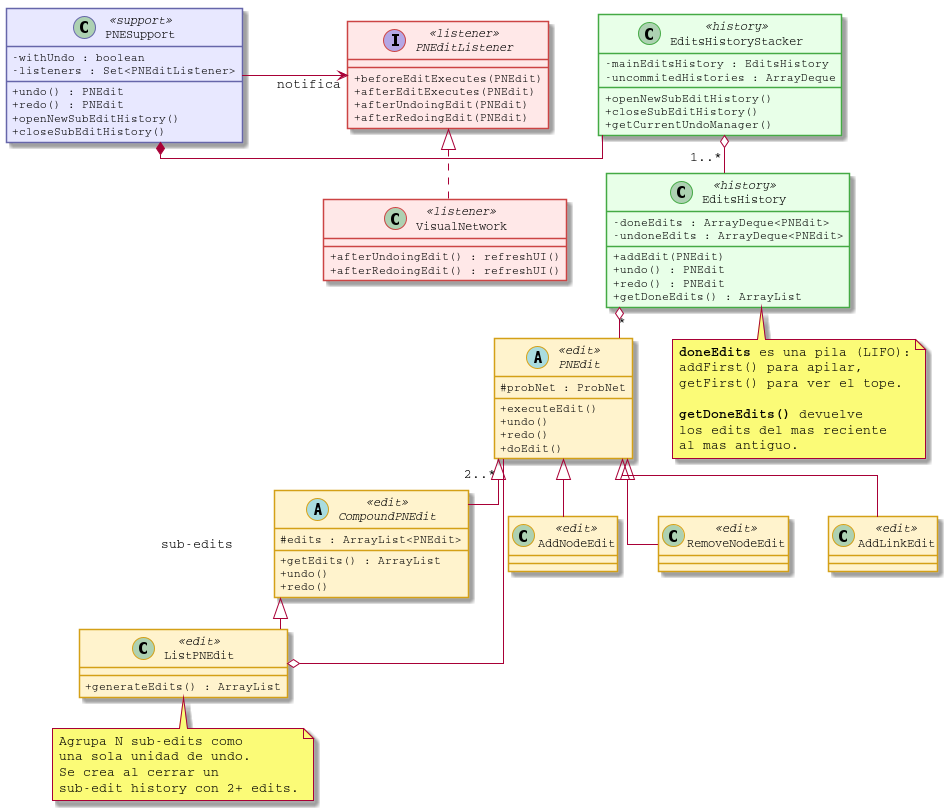
\includegraphics[width=\textwidth]{diagrams/arquitectura-undo-redo.png}
  \caption{Clases principales del sistema de undo/redo.}
  \label{fig:arquitectura}
\end{figure}


\subsection{Clases clave}

\begin{description}[style=nextline, leftmargin=2em]
\raggedright

\item[\clase{PNESupport}]
  Punto de entrada para undo/redo. Mantiene el conjunto de listeners
  (\clase{PNEditListener}) y los métodos \metodo{undo()} y \metodo{redo()},
  que delegan en el historial y notifican a los listeners.

\item[\clase{EditsHistoryStacker}]
  Gestiona una pila de historiales. Permite abrir sub-historiales anidados
  (transacciones) con \metodo{openNewSubEditHistory()} y cerrarlos con
  \metodo{closeSubEditHistory()}. Al cerrar un sub-historial con dos o más
  edits, los empaqueta en un \clase{ListPNEdit}.

\item[\clase{EditsHistory}]
  Un historial individual con dos pilas: \code{doneEdits} (edits ejecutados)
  y \code{undoneEdits} (edits deshechos). Ambas son \clase{ArrayDeque} usadas
  como pilas LIFO: los edits se apilan con \metodo{addFirst()} y se
  consultan con \metodo{getFirst()}.

\item[\clase{CompoundPNEdit}]
  Edit abstracto que contiene una lista de sub-edits. Su \metodo{redo()}
  ejecuta los sub-edits en orden directo; su \metodo{undo()} los ejecuta
  en orden inverso.

\item[\clase{ListPNEdit}]
  Implementación concreta de \clase{CompoundPNEdit} que simplemente almacena
  la lista de sub-edits que recibe en el constructor.

\item[\clase{PNEditListener}]
  Interfaz de observador con cuatro métodos: \metodo{beforeEditExecutes},
  \metodo{afterEditExecutes}, \metodo{afterUndoingEdit} y
  \metodo{afterRedoingEdit}.

\end{description}


\subsection{Flujo normal de una edición compuesta}

Para entender los bugs, es útil seguir el flujo completo de una edición
compuesta. Supongamos que el usuario ejecuta una acción que crea dos nodos
(A y B) y un arco entre ellos (A$\to$B):

\begin{enumerate}
  \item La GUI llama a \metodo{openNewSubEditHistory()}.
        Esto crea un nuevo \clase{EditsHistory} vacío en la pila.

  \item Se ejecutan los edits individuales:
        \begin{itemize}
          \item \code{AddNodeEdit(A).executeEdit()} --- se añade a la pila:
                \code{doneEdits = [A]}
          \item \code{AddNodeEdit(B).executeEdit()} --- se apila encima:
                \code{doneEdits = [B, A]}
          \item \code{AddLinkEdit(A$\to$B).executeEdit()} --- se apila encima:
                \code{doneEdits = [Link, B, A]}
        \end{itemize}
        Cada uno notifica a los listeners con \metodo{afterEditExecutes}.

  \item La GUI llama a \metodo{pneSupport.closeSubEditHistory()}.
        \clase{EditsHistoryStacker} obtiene los \code{doneEdits} del
        sub-historial y los empaqueta en un \clase{ListPNEdit}.

  \item El \clase{ListPNEdit} se añade al historial padre como un solo edit.
\end{enumerate}

El punto crítico es el paso 3: \metodo{getDoneEdits()} devuelve los edits
en \textbf{orden de pila} (el más reciente primero), es decir
\textbf{[Link, B, A]}. Este es el orden en que se almacenan dentro del
\clase{ListPNEdit}.

\medskip

La Figura~\ref{fig:pila} muestra paso a paso cómo evoluciona la pila
\code{doneEdits} durante la ejecución de los tres edits, y cómo la lectura
de la pila produce una lista en orden inverso al de ejecución --- la causa
raíz del Bug~3.

\begin{figure}[H]
  \centering
  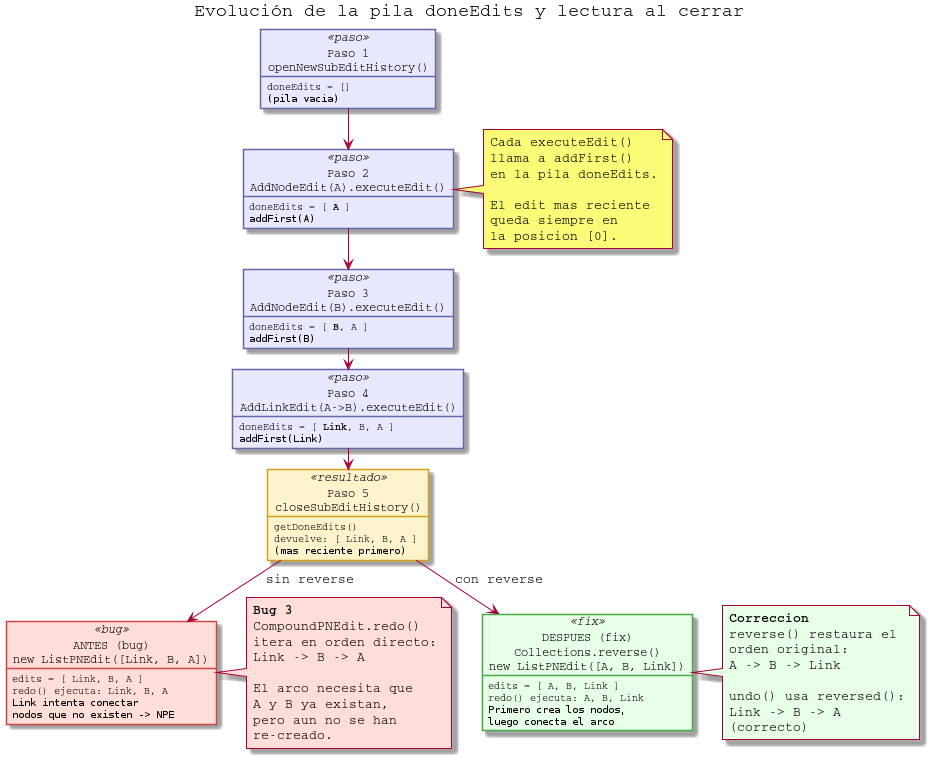
\includegraphics[width=\textwidth]{diagrams/pila-edits.png}
  \caption{Evolución de la pila \code{doneEdits} durante la ejecución.
           Cada \metodo{executeEdit()} apila el edit con \metodo{addFirst()}.
           Al cerrar el sub-historial, \metodo{getDoneEdits()} devuelve la
           lista en orden de pila (más reciente primero). Sin el
           \metodo{reverse()}, el \clase{ListPNEdit} almacena los edits en
           orden invertido.}
  \label{fig:pila}
\end{figure}

% =====================================================================
\section{Los tres bugs}
\label{sec:bugs}
% =====================================================================


\subsection{Bug 1: Notificaciones duplicadas en redo}
\label{sec:bug1}

\subsubsection{Síntoma}

Al rehacer un compound edit, los listeners recibían \textbf{tres}
notificaciones \metodo{afterRedoingEdit} en vez de una: una con el
\clase{ListPNEdit} y una con cada sub-edit.

\subsubsection{Causa}

El método \metodo{PNESupport.redo()} utilizaba un método auxiliar
\metodo{flattenEdit()} que expandía recursivamente el compound edit en una
lista plana mediante BFS (búsqueda en anchura). Dado un \clase{ListPNEdit}
con sub-edits [B, A], \metodo{flattenEdit()} devolvía:

\begin{center}
\code{[ListPNEdit, B, A]}
\end{center}

Y luego iteraba esta lista, notificando a cada listener con cada elemento.
El resultado era que el listener recibía la notificación para el compound
\emph{y también} para cada sub-edit individual.

\subsubsection{Código con el bug}

\begin{lstlisting}[caption={Método \metodo{redo()} con el bug (simplificado).},
  label=lst:redo-antes]
public ArrayList<PNEdit> redo() {
    var redoneEdit = editsHistoryStacker
        .getCurrentUndoManager().redo();
    // flattenEdit() devuelve [compound, subA, subB]
    ArrayList<PNEdit> redoneEdits = flattenEdit(redoneEdit);
    for (PNEdit subRedoneEdit : redoneEdits) {
        for (PNEditListener listener : listeners) {
            listener.afterRedoingEdit(subRedoneEdit);
        }
    }
    return redoneEdits;
}
\end{lstlisting}

\begin{lstlisting}[caption={Método \metodo{flattenEdit()} --- BFS que causa la duplicación.},
  label=lst:flatten]
private ArrayList<PNEdit> flattenEdit(PNEdit edit) {
    var editsToVisit = new ArrayDeque<PNEdit>();
    editsToVisit.addFirst(edit);
    var flattenedEdits = new ArrayList<PNEdit>();
    while (!editsToVisit.isEmpty()) {
        var e = editsToVisit.removeFirst();
        flattenedEdits.add(e);
        if (e instanceof CompoundPNEdit compound) {
            compound.getEdits()
                    .forEach(editsToVisit::addLast);
        }
    }
    return flattenedEdits;
}
\end{lstlisting}


\subsection{Bug 2: Evento asimétrico en redo}
\label{sec:bug2}

\subsubsection{Síntoma}

Durante la ejecución original, los listeners recibían
\metodo{afterEditExecutes(compound)}. Pero en un redo, debido a
\metodo{flattenEdit()}, recibían \metodo{afterRedoingEdit(subEdit)} para
cada sub-edit individual. Esto creaba una \textbf{asimetría}: el listener
tenía que manejar dos tipos de evento distintos para la misma operación
lógica.

\subsubsection{Causa}

La misma que el Bug~1: \metodo{flattenEdit()} descomponía el compound en
sus partes, y cada parte se notificaba con \metodo{afterRedoingEdit} en vez
de notificar una sola vez con el edit completo.


\subsection{Bug 3: Orden incorrecto de sub-edits en compound}
\label{sec:bug3}

\subsubsection{Síntoma}

Al rehacer un compound edit que contenía edits dependientes (por ejemplo,
crear un nodo y luego crear un arco hacia ese nodo), el redo fallaba con
\code{NullPointerException} porque intentaba rehacer el arco antes de que
el nodo existiera.

\subsubsection{Causa}

La pila \code{doneEdits} de \clase{EditsHistory} almacena los edits con
\metodo{addFirst()}, es decir, el más reciente queda primero. El método
\metodo{getDoneEdits()} simplemente copia esta pila en un \clase{ArrayList},
devolviendo los edits en \textbf{orden inverso} al de ejecución original.

Este \clase{ArrayList} se pasaba directamente al constructor de
\clase{ListPNEdit}, que lo almacenaba tal cual. El resultado:

\begin{itemize}
  \item El usuario ejecuta: A, B, Link(A$\to$B)
  \item \code{getDoneEdits()} devuelve: [Link, B, A]
  \item \clase{ListPNEdit} almacena: [Link, B, A]
\end{itemize}

\clase{CompoundPNEdit} ejecuta \metodo{redo()} en orden directo sobre esta
lista, y \metodo{undo()} en orden inverso:

\begin{lstlisting}[caption={Métodos \metodo{redo()} y \metodo{undo()} de
  \clase{CompoundPNEdit}.}, label=lst:compound]
@Override public void redo() {
    this.getEdits().forEach(PNEdit::redo);
}

@Override public void undo() {
    this.getEdits().reversed().forEach(PNEdit::undo);
}
\end{lstlisting}

Con la lista [Link, B, A]:
\begin{itemize}
  \item \textbf{redo()} ejecuta: Link.redo(), B.redo(), A.redo() ---
        \textbf{incorrecto}: el arco se rehace antes que los nodos.
        Si el arco depende de los nodos, se produce un
        \code{NullPointerException}.
  \item \textbf{undo()} ejecuta \code{reversed()}: A.undo(), B.undo(),
        Link.undo() --- \textbf{incorrecto}: los nodos se deshacen antes
        que el arco.
\end{itemize}

\subsubsection{Por qué no se manifestaba siempre}

Con edits independientes (por ejemplo, dos \code{AddNodeEdit} sin arcos
entre ellos), el orden de ejecución no importa y el undo/redo funciona
correctamente. El bug solo se manifestaba con edits dependientes, como
crear un arco entre dos nodos recién creados.

\medskip

La Figura~\ref{fig:orden} ilustra el problema del orden con un ejemplo
concreto.

\begin{figure}[H]
  \centering
  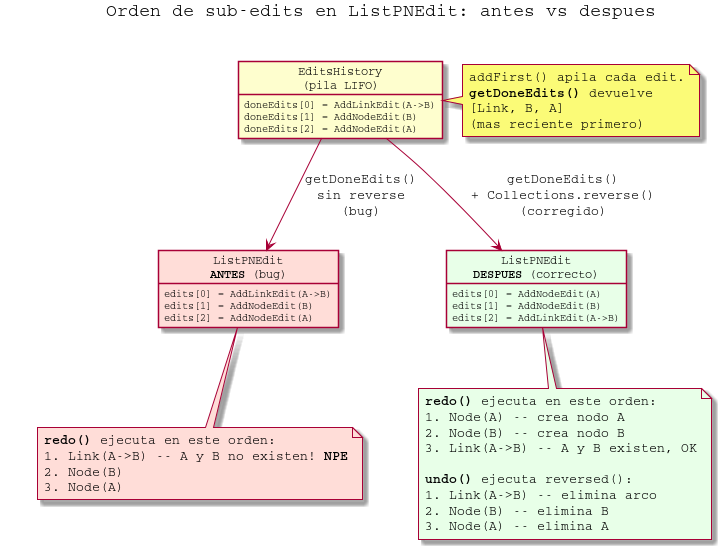
\includegraphics[width=\textwidth]{diagrams/orden-edits.png}
  \caption{Orden de sub-edits dentro de \clase{ListPNEdit}: antes (bug) y después (correcto).}
  \label{fig:orden}
\end{figure}


% =====================================================================
\section{Corrección aplicada}
\label{sec:fix}
% =====================================================================

La corrección consta de dos cambios independientes, cada uno dirigido a una
causa raíz distinta.


\subsection{Cambio 1: Eliminar \metodo{flattenEdit()} (Bugs 1 y 2)}

Se eliminó el método \metodo{flattenEdit()} y se simplificaron
\metodo{undo()} y \metodo{redo()} para notificar una sola vez con el edit
que devuelve \clase{EditsHistory}:

\begin{lstlisting}[caption={Método \metodo{redo()} corregido.},
  label=lst:redo-despues, backgroundcolor=\color{fixbg}]
public @Nullable PNEdit redo() {
    var redoneEdit = editsHistoryStacker
        .getCurrentUndoManager().redo();
    if (redoneEdit != null) {
        for (PNEditListener listener : listeners) {
            listener.afterRedoingEdit(redoneEdit);
        }
    }
    return redoneEdit;
}
\end{lstlisting}

\begin{lstlisting}[caption={Método \metodo{undo()} corregido.},
  label=lst:undo-despues, backgroundcolor=\color{fixbg}]
public @Nullable PNEdit undo() {
    var undoneEdit = editsHistoryStacker
        .getCurrentUndoManager().undo();
    if (undoneEdit != null) {
        for (PNEditListener listener : listeners) {
            listener.afterUndoingEdit(undoneEdit);
        }
    }
    return undoneEdit;
}
\end{lstlisting}

\textbf{Consecuencias:}
\begin{itemize}
  \item Para un edit simple, el comportamiento no cambia: el listener recibe
        una notificación con el edit.
  \item Para un compound edit, el listener recibe una sola notificación con
        el \clase{ListPNEdit}. Si necesita los sub-edits, puede hacer
        \code{instanceof CompoundPNEdit} y llamar a \metodo{getEdits()}.
  \item Se eliminaron las anotaciones \code{@ToCheck} de ambos métodos.
  \item El tipo de retorno cambió de \code{ArrayList<PNEdit>} a
        \code{@Nullable PNEdit}. Se actualizaron los dos llamadores que
        usaban el valor de retorno (ver Sección~\ref{sec:callers}).
\end{itemize}


\subsection{Cambio 2: Invertir el orden de \metodo{getDoneEdits()} (Bug 3)}

En el método \metodo{closeSubEditHistory()} de la clase
\clase{EditsHistoryStacker}, se añadió una llamada a
\metodo{Collections.reverse()} después de obtener los \code{doneEdits},
para restaurar el orden original de ejecución antes de pasarlo al
constructor de \clase{ListPNEdit}:

\begin{lstlisting}[caption={\metodo{closeSubEditHistory()} corregido (fragmento).},
  label=lst:close-despues, backgroundcolor=\color{fixbg}]
var lastUsedStack = this.uncommitedHistories.removeLast();
// getDoneEdits() devuelve el mas reciente primero (pila);
// invertimos para restaurar el orden original de ejecución.
ArrayList<PNEdit> doneEdits = lastUsedStack.getDoneEdits();
Collections.reverse(doneEdits);
PNEdit stackAsEdit = switch (doneEdits.size()) {
    case 0 -> null;
    case 1 -> doneEdits.getFirst();
    default -> new ListPNEdit(
        doneEdits.getFirst().getProbNet(), doneEdits);
};
\end{lstlisting}

Con esta corrección, si el usuario ejecutó A, B, Link(A$\to$B):
\begin{itemize}
  \item \code{getDoneEdits()} devuelve: [Link, B, A]
  \item Tras \code{reverse()}: [A, B, Link]
  \item \clase{ListPNEdit} almacena: [A, B, Link]
  \item \metodo{redo()} ejecuta: A, B, Link --- \textbf{correcto}
  \item \metodo{undo()} ejecuta \code{reversed()}: Link, B, A --- \textbf{correcto}
\end{itemize}


\subsection{Actualización de llamadores}
\label{sec:callers}

El cambio de tipo de retorno de \metodo{undo()} y \metodo{redo()} (de
\code{ArrayList<PNEdit>} a \code{@Nullable PNEdit}) requirió actualizar
dos llamadores que usaban el valor de retorno:

\begin{table}[H]
\centering
\caption{Llamadores actualizados por el cambio de tipo de retorno.}
\label{tab:callers}
\small
\begin{tabularx}{\textwidth}{lX}
\toprule
\textbf{Clase} & \textbf{Cambio} \\
\midrule
\code{EditsHistoryPlugin} \newline
\footnotesize{(org.openmarkov.full)} &
Usaba \code{.undo().contains(edit)} en un bucle \code{while}.
Cambiado a un bucle \code{do-while} que compara el edit devuelto con \code{equals()}. \\
\addlinespace
\code{EditorInputHandler} \newline
\footnotesize{(org.openmarkov.gui)} &
Usaba \code{.undo().stream().anyMatch(...)}.
Cambiado a un bucle \code{do-while} que comprueba \code{instanceof AddNodeEdit}. \\
\bottomrule
\end{tabularx}
\end{table}

\medskip

Todos los demás llamadores (más de 20 en GUI, tests y learning) usaban
\metodo{undo()}/\metodo{redo()} sin capturar el valor de retorno, por lo que
no requirieron cambios.


% =====================================================================
\section{Diagramas de secuencia: antes y después}
\label{sec:diagramas}
% =====================================================================

Las Figuras~\ref{fig:flujo-antes} y~\ref{fig:flujo-despues} muestran el
flujo de ejecución de \metodo{redo()} con un compound edit, antes y después
de la corrección.

\begin{figure}[H]
  \centering
  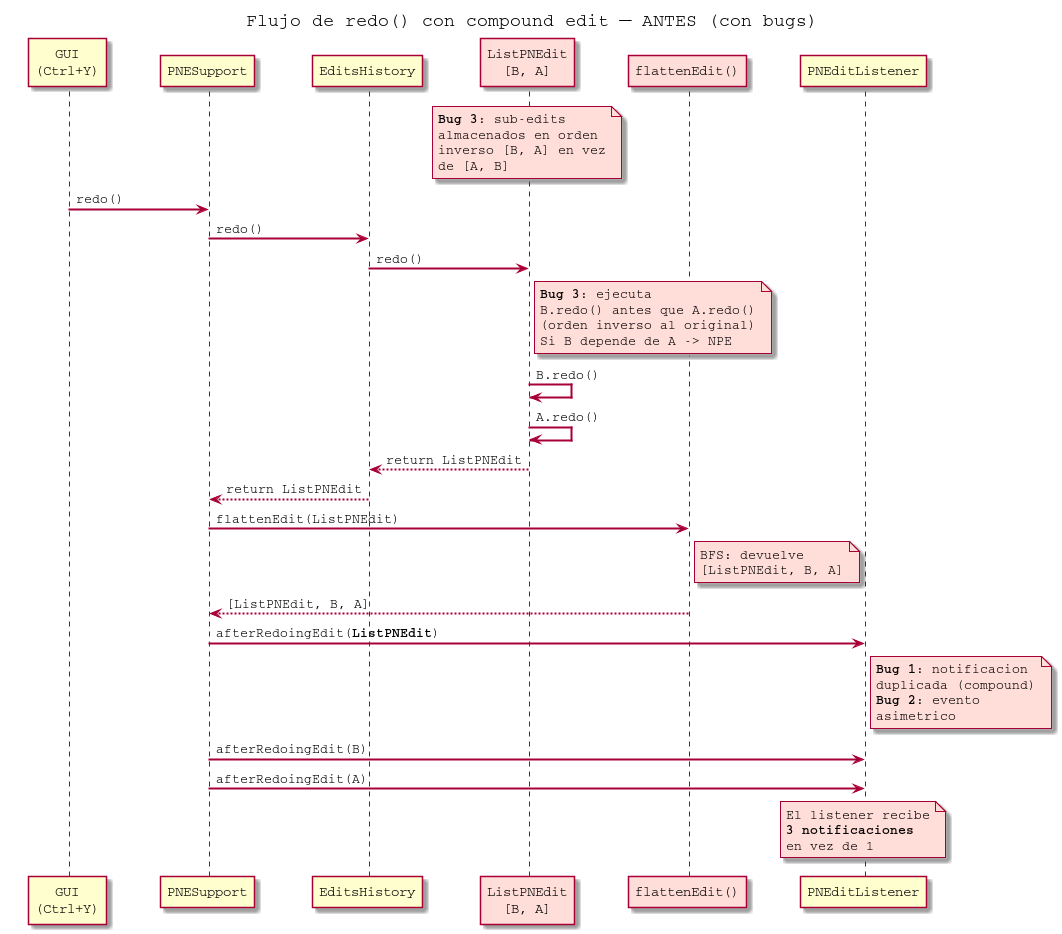
\includegraphics[width=0.85\textwidth]{diagrams/flujo-antes.png}
  \caption{Flujo de \metodo{redo()} \textbf{antes} de la corrección. Se observan
           los tres bugs: orden incorrecto (Bug~3), notificaciones duplicadas (Bug~1)
           y evento asimétrico (Bug~2).}
  \label{fig:flujo-antes}
\end{figure}

\begin{figure}[H]
  \centering
  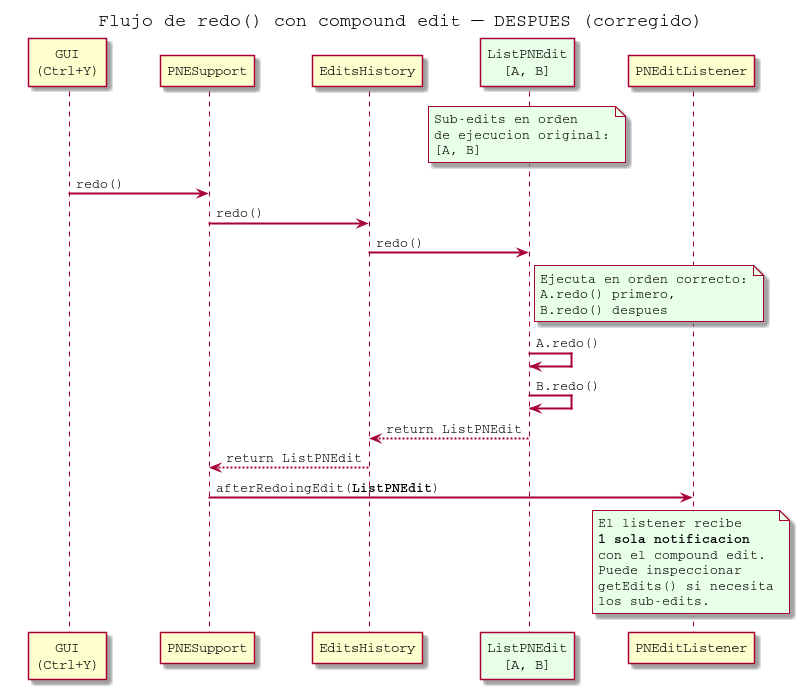
\includegraphics[width=0.85\textwidth]{diagrams/flujo-despues.png}
  \caption{Flujo de \metodo{redo()} \textbf{después} de la corrección. Los sub-edits
           se ejecutan en orden correcto y el listener recibe una única notificación.}
  \label{fig:flujo-despues}
\end{figure}


% =====================================================================
\section{Ejemplo completo}
\label{sec:ejemplo}
% =====================================================================

Para ilustrar el impacto práctico, consideremos el siguiente escenario real
en la GUI:

\begin{enumerate}
  \item El usuario abre el diálogo de propiedades de un nodo B.
  \item Añade un padre A (se ejecuta \code{AddNodeEdit(A)} y
        \code{AddLinkEdit(A$\to$B)}).
  \item Pulsa Aceptar (se cierra el sub-historial).
  \item Pulsa Ctrl+Z (undo): se deshace todo correctamente.
  \item Pulsa Ctrl+Y (redo).
\end{enumerate}

\subsection{Comportamiento antes de la corrección}

En el paso~5, \metodo{redo()} ejecutaba los sub-edits del \clase{ListPNEdit}
en orden de pila: primero \code{AddLinkEdit(A$\to$B)}, luego
\code{AddNodeEdit(A)}. El arco intentaba conectar dos nodos que aún no
existían, produciendo:

\begin{lstlisting}[language={},frame=single,backgroundcolor=\color{bugbg},
  numbers=none,basicstyle=\ttfamily\small]
NullPointerException: Cannot invoke
  "Node.setPotentials(List)"
  because "this.nodeTo" is null
\end{lstlisting}

\subsection{Comportamiento después de la corrección}

En el paso~5, \metodo{redo()} ejecuta los sub-edits en orden original:
primero \code{AddNodeEdit(A)}, luego \code{AddLinkEdit(A$\to$B)}. El nodo A
existe cuando se crea el arco. El redo completa sin error y la red queda en
el mismo estado que tras el paso~2.


% =====================================================================
\section{Tests de regresión}
\label{sec:tests}
% =====================================================================

Se creó la clase \code{PNESupportPropertyTest} con 7 tests usando jqwik
(\code{@Property} y \code{@Example}):

\begin{table}[H]
\centering
\caption{Tests de regresión para el sistema de undo/redo.}
\label{tab:tests}
\small
\begin{tabularx}{\textwidth}{lX}
\toprule
\textbf{Test} & \textbf{Qué verifica} \\
\midrule
\code{simpleEdit\_undoNotifies\-ListenerExactlyOnce} &
  Undo de un edit simple produce exactamente una notificación. \\
\addlinespace
\code{simpleEdit\_redoNotifies\-ListenerExactlyOnce} &
  Redo de un edit simple produce exactamente una notificación. \\
\addlinespace
\code{simpleEdit\_undoRedo\-PreservesNetworkState} &
  Tras undo + redo de un edit simple, el estado de la red es idéntico
  al original. \\
\addlinespace
\code{compoundEdit\_undoRedo\-NotifiesExactlyOnce} &
  Undo y redo de un compound edit producen exactamente una notificación cada
  uno, y la notificación lleva el \clase{CompoundPNEdit}. \textbf{Regresión
  para Bugs 1 y 2.} \\
\addlinespace
\code{compoundEdit\_subEdits\-InOriginalOrder} &
  Los sub-edits dentro del \clase{ListPNEdit} están en el orden original
  de ejecución. \textbf{Regresión para Bug 3.} \\
\addlinespace
\code{compoundEdit\_redo\-DependentEditsDoesNotThrow} &
  Redo de un compound con edits dependientes (nodos + arco) no lanza
  excepción. \textbf{Regresión para Bug 3.} \\
\addlinespace
\code{compoundEdit\_undoRedo\-PreservesNetworkState} &
  Tras undo + redo de un compound con edits dependientes, la red conserva
  todos los nodos y arcos. \\
\bottomrule
\end{tabularx}
\end{table}

Todos los tests pasan con la corrección aplicada y fallan sin ella, lo que
confirma tanto la existencia de los bugs como la corrección.


% =====================================================================
\section{Resumen de ficheros modificados}
% =====================================================================

\begin{table}[H]
\centering
\caption{Ficheros modificados en la corrección.}
\label{tab:ficheros}
\small
\begin{tabularx}{\textwidth}{llX}
\toprule
\textbf{Módulo} & \textbf{Fichero} & \textbf{Cambio} \\
\midrule
core & \code{PNESupport.java} &
  Eliminados \metodo{flattenEdit()} y \code{@ToCheck}.
  Tipo de retorno de \metodo{undo()}/\metodo{redo()} cambiado a
  \code{@Nullable PNEdit}. Notificación única. \\
\addlinespace
core & \code{EditsHistoryStacker.java} &
  Añadido \code{Collections.reverse(doneEdits)} en
  \metodo{closeSubEditHistory()}. \\
\addlinespace
full & \code{EditsHistoryPlugin.java} &
  Adaptado al nuevo tipo de retorno. \\
\addlinespace
gui & \code{EditorInputHandler.java} &
  Adaptado al nuevo tipo de retorno. \\
\addlinespace
core (test) & \code{PNESupportPropertyTest.java} &
  7 tests de regresión (nuevo fichero). \\
\bottomrule
\end{tabularx}
\end{table}


% =====================================================================
\section{Impacto en la GUI}
% =====================================================================

El principal listener de undo/redo en la GUI es \clase{VisualNetwork}, que
implementa los métodos de notificación de undo y redo con una llamada a
\metodo{refreshUI()} que repinta toda la vista. Este listener es tolerante
a notificaciones duplicadas o en orden incorrecto, ya que siempre repinta
completamente. Por esta razón, los bugs no causaban problemas visibles en
la mayoría de los casos de uso.

\medskip

Sin embargo, otros listeners (\clase{ValuesTable}, \clase{ICIValuesTable},
constraints como \clase{NoCycle}) podrían haberse visto afectados por
notificaciones duplicadas o en orden incorrecto. Además, el Bug~3 causaba
un \code{NullPointerException} irrecuperable al rehacer compound edits con
dependencias, lo que sí era un fallo visible para el usuario.


\end{document}
